
\tikzset{
    vertex/.style = {
        circle,
        fill            = black,
        outer sep = 2pt,
        inner sep = 1pt,
    }
}
\begin{figure}[H]

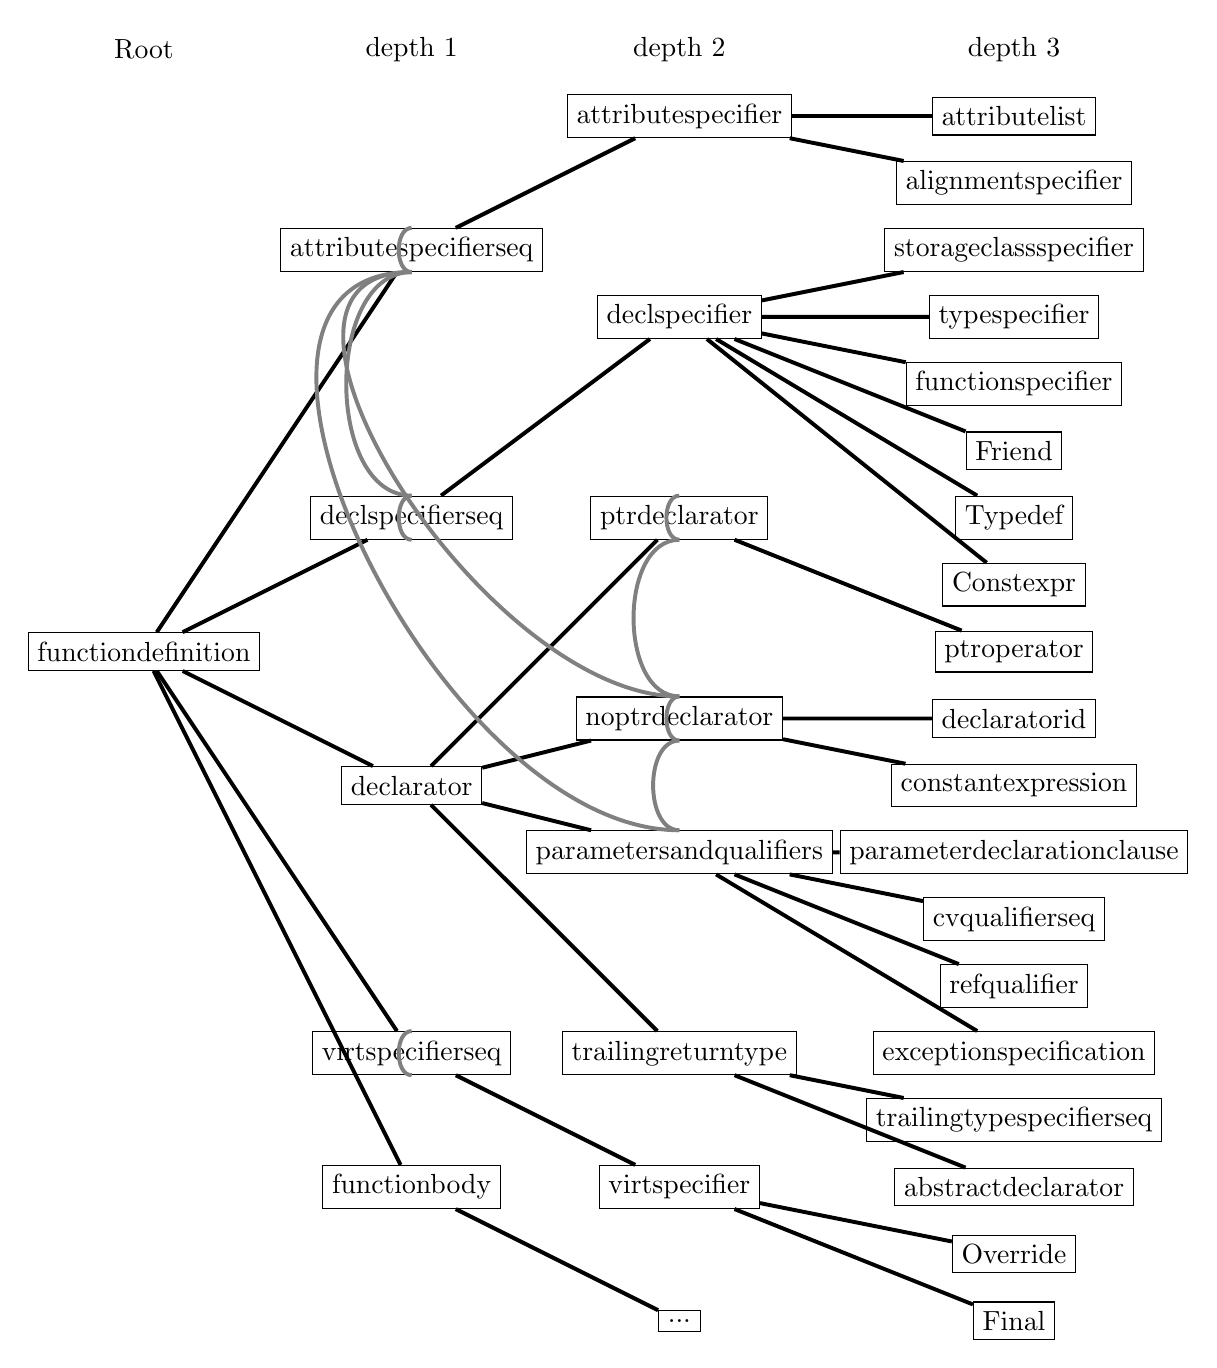
\begin{tikzpicture}[scale=0.85]
    % root
    \node at (0.0, 1.0) {Root};
    \node[draw] (funcDef) at (0.0, -8.0) {functiondefinition};
    
    %level1
    \node at (4, 1.0) {depth 1}; 
    \node[draw] (attribSeq) at (4, -2) {attributespecifierseq};
    \node[draw] (declSeq) at (4, -6.0) {declspecifierseq};
    \node[draw] (decl) at (4, -10.0) {declarator};
    \node[draw] (virtSeq) at (4, -14.0) {virtspecifierseq};
    \node[draw] (funcBody) at (4, -16.0) {functionbody};
    
    %root - level1
    \draw[line width=0.5mm,draw=black] (funcDef) to (attribSeq);
    \draw[line width=0.5mm,draw=black] (funcDef) to (declSeq);
    \draw[line width=0.5mm,draw=black] (funcDef) to (decl);
    \draw[line width=0.5mm,draw=black] (funcDef) to (virtSeq);
    \draw[line width=0.5mm,draw=black] (funcDef) to (funcBody);
    
    %level1 to exist
    \draw[line width=0.5mm,draw=gray] (attribSeq.south) to[in=180,out=180] (attribSeq.north);
    \draw[line width=0.5mm,draw=gray] (declSeq.north) to[in=180,out=180] (attribSeq.south);
    \draw[line width=0.5mm,draw=gray] (declSeq.south) to[in=180,out=180] (declSeq.north);
    \draw[line width=0.5mm,draw=gray] (virtSeq.south) to[in=180,out=180] (virtSeq.north);
    
    % level2
    \node at (8.0, 1.0) {depth 2};
    \node[draw] (attrib) at (8.0, -0.0) {attributespecifier};
    \node[draw] (declSpec) at (8.0, -3.0) {declspecifier};
    \node[draw] (ptrDecl) at (8.0, -6.0) {ptrdeclarator};
    \node[draw] (noptrDecl) at (8.0, -9.0) {noptrdeclarator};
    \node[draw] (param&qual) at (8.0, -11.0) {parametersandqualifiers};
    \node[draw] (trailReturn) at (8.0, -14.0) {trailingreturntype};
    \node[draw] (virtSpec) at (8.0, -16.0) {virtspecifier};
    \node[draw] (toMuch) at (8.0, -18.0) {...};
    
    %level1 - level2
    \draw[line width=0.5mm,draw=black] (attribSeq) to (attrib);
    \draw[line width=0.5mm,draw=black] (declSeq) to (declSpec);
    \draw[line width=0.5mm,draw=black] (decl) to (ptrDecl);
    \draw[line width=0.5mm,draw=black] (decl) to (noptrDecl);
    \draw[line width=0.5mm,draw=black] (decl) to (param&qual);
    \draw[line width=0.5mm,draw=black] (decl) to (trailReturn);
    \draw[line width=0.5mm,draw=black] (virtSeq) to (virtSpec);
    \draw[line width=0.5mm,draw=black] (funcBody) to (toMuch);
    
    %level2 to exist
    \draw[line width=0.5mm,draw=gray] (ptrDecl.south) to[in=180,out=180] (noptrDecl.north);
    \draw[line width=0.5mm,draw=gray] (ptrDecl.south) to[in=180,out=180] (ptrDecl.north);
    \draw[line width=0.5mm,draw=gray] (noptrDecl.north) to[in=180,out=180] (attribSeq.south);
    \draw[line width=0.5mm,draw=gray] (noptrDecl.south) to[in=180,out=180] (param&qual.north);
    \draw[line width=0.5mm,draw=gray] (noptrDecl.south) to[in=180,out=180] (noptrDecl.north);
    \draw[line width=0.5mm,draw=gray] (param&qual.north) to[in=180,out=180] (attribSeq.south);
    
    % level3
    \node at (13.0, 1.0) {depth 3};
    \node[draw] (attribList) at (13.0, -0.0) {attributelist};
    \node[draw] (alignmentspecifier) at (13.0, -1.0) {alignmentspecifier};
    \node[draw] (storageclassspecifier) at (13.0, -2.0) {storageclassspecifier};
    \node[draw] (typespecifier) at (13.0, -3.0) {typespecifier};
    \node[draw] (functionspecifier) at (13.0, -4.0) {functionspecifier};
    \node[draw] (Friend) at (13.0, -5.0) {Friend};
    \node[draw] (Typedef) at (13.0, -6.0) {Typedef};
    \node[draw] (Constexpr) at (13.0, -7.0) {Constexpr};
    \node[draw] (ptroperator) at (13.0, -8.0) {ptroperator};
    \node[draw] (declaratorid) at (13.0, -9.0) {declaratorid};
    \node[draw] (constantexpression) at (13.0, -10.0) {constantexpression};
    \node[draw] (parameterdeclarationclause) at (13.0, -11.0) {parameterdeclarationclause};
    \node[draw] (cvqualifierseq) at (13.0, -12.0) {cvqualifierseq};
    \node[draw] (refqualifier) at (13.0, -13.0) {refqualifier};
    \node[draw] (exceptionspecification) at (13.0, -14.0) {exceptionspecification};
    \node[draw] (trailingtypespecifierseq) at (13.0, -15.0) {trailingtypespecifierseq};
    \node[draw] (abstractdeclarator) at (13.0, -16.0) {abstractdeclarator};
    \node[draw] (Override) at (13.0, -17.0) {Override};
    \node[draw] (Final) at (13.0, -18.0) {Final};

    
    %level2 - level3
    \draw[line width=0.5mm,draw=black] (attrib) to (alignmentspecifier);
    \draw[line width=0.5mm,draw=black] (attrib) to (attribList);
    \draw[line width=0.5mm,draw=black] (declSpec) to (storageclassspecifier);
    \draw[line width=0.5mm,draw=black] (declSpec) to (typespecifier);
    \draw[line width=0.5mm,draw=black] (declSpec) to (functionspecifier);
    \draw[line width=0.5mm,draw=black] (declSpec) to (Friend);
    \draw[line width=0.5mm,draw=black] (declSpec) to (Typedef);
    \draw[line width=0.5mm,draw=black] (declSpec) to (Constexpr);
    \draw[line width=0.5mm,draw=black] (ptrDecl) to (ptroperator);
    \draw[line width=0.5mm,draw=black] (noptrDecl) to (declaratorid);
    \draw[line width=0.5mm,draw=black] (noptrDecl) to (constantexpression);
    \draw[line width=0.5mm,draw=black] (param&qual) to (parameterdeclarationclause);
    \draw[line width=0.5mm,draw=black] (param&qual) to (cvqualifierseq);
    \draw[line width=0.5mm,draw=black] (param&qual) to (refqualifier);
    \draw[line width=0.5mm,draw=black] (param&qual) to (exceptionspecification);
    \draw[line width=0.5mm,draw=black] (trailReturn) to (trailingtypespecifierseq);
    \draw[line width=0.5mm,draw=black] (trailReturn) to (abstractdeclarator);
    \draw[line width=0.5mm,draw=black] (virtSpec) to (Override);
    \draw[line width=0.5mm,draw=black] (virtSpec) to (Final);

    

\end{tikzpicture}

    \caption{CPP functiondefinition graph to depth 3}
    \medskip
    \small
    Straight lines show that the, right-hand side is contained within the left side.
    Curved lines show that something defined earlier or at the same level is also within the rule.
    \label{CPPFunctionDefinition}
\end{figure}

